\section{Sorption}

Exchange processes, like sorption, between the solid and the liquid phase in the multiphase system of an aquifer can be caused by physical (Van-der-Waals-forces) or chemical bonds. Sorption processes can be reversible (adsorption-desorption) if the chemical environment is changing. When the transport in a multiphase system is simulated, the mass exchange between the liquid and the solid phase has to be included. The equations that describe the sorption processes are called sorption isotherms. Sorption isotherms describe the relation between the substance that is adsorbed on the solid matrix and the one which is dissolved in the fluid phase. Those equations are only valid under isothermal conditions. The isotherms that are listed below, base on the assumption that the adsorbed substance and the dissolved one are in the state of equilibrium.

\begin{eqnarray}
\mathrm{Henry:}
& \qquad &
S\,=\,K_D\cdot C \\[2.0ex]
\label{eq58}
%
\mathrm{Freundlich:}
& \qquad &
S\,=\,K_1\cdot C^{K_2} \\[2.0ex]
\label{eq59}
%
\mathrm{Langmuir:\hspace*{0.8ex}}
& \qquad &
S\,=\,\frac{K_1\cdot C}{1+K_2\cdot C}
\label{eq510}
\end{eqnarray}

{\small
with
\begin{tabbing}
\=xxxxxxxxxxxx \=xxxxxxxxxxxxxxxxxx \kill
\> $K_D,\; K_1,\; K_2$ \> - distribution coefficients, \\[1.0ex]
\> $S$ \> - concentration of the adsorbed species (kg/kg), \\[1.0ex]
\> $C$ \> - concentration of the dissolved species (kg/m$^3$).
\end{tabbing}
}

The distribution coefficients are dependent on the substance and the specific soil properties like the pH. The linear Henry-isotherm is often used when there are low concentrations. Non-linear sorption processes are reproduced by the Freundlich or the Langmuir isotherm. Then the retardation is dependent on the solute concentration. In addition, the use of the Langmuir isotherm assumes a constant amount of sorption space at the solid surface. A maximum concentration for the adsorbed substance on the solid matrix is exclusively considered by the Langmuir isotherm \cite{Hab:01}. This maximum concentration $c_{\mathrm{max}}$ is included in the distribution coefficient $K_1$ ($K_1=c_{\mathrm{max}}\cdot K_2$). The distribution coefficient $K_2$ of the Langmuir isotherm stands for the affinity between solid and sorbed solute. The distribution coefficients do not have comparable values: each sorption isotherm has to be considered separately with its specific constants.

%----------
\subsection{Linear sorption (Henry isotherm)}

The aim of this example is to simulate the solute transport in an aquifer by convection with the influence of retardation as a result of sorption. The solute transport is influenced by linear sorption processes. That means, the Henry-isotherm is relevant to calculate the solute concentration. The calculation area and boundary conditions are the same as described for the precedent example.

The following simplifications are assumed: (1) exclusively linear sorption (Henry isotherm), no decay of components (2) homogeneous aquifer, saturated, stationary flow (Fig. \ref{fig51}).
%
The soil parameters are the same as listed in Table \ref{tab51}, but decay is not considered during these simulation runs. For the different simulation runs the Henry-sorption coefficients are varied as listed in Table \ref{tab52} in order to evaluate the influence of sorption on the mass transport. The retardation coefficients $R$ are calculated by solving equation (\ref{eq52}).

\begin{table}[h]%[tab-ldhp]
\begin{center}
\begin{tabular}{ll}
\toprule
K$_D$ value [m$^3$/kg] & Retardation coefficient [-] \\
\midrule
0  & 1  \\			
6.8 $\cdot 10^{-6}$ & 1.05 \\
6.8 $\cdot 10^{-5}$ & 1.54  \\
6.8 $\cdot 10^{-4}$ & 6.44  \\
\bottomrule
\end{tabular}
\caption{Variation of K$_D$-values and retardation coefficients as input variables}
\label{tab52}
\end{center}
\end{table}

\subsubsection{Results}

The concentration distribution at a special point in time and over a given distance is calculated by equation (\ref{eq53}). Hereby the decay term $\gamma$ is set equal to 1. The analytical solutions are depicted in Figure \ref{fig53} as single symbols.
%
In Figure \ref{fig53} you can find the concentration distribution over the whole length of the 1~D model at the final simulation time of 100 days. Obviously, the numerical results meet well the analytical solutions.

\begin{figure}[htbp]
\centering
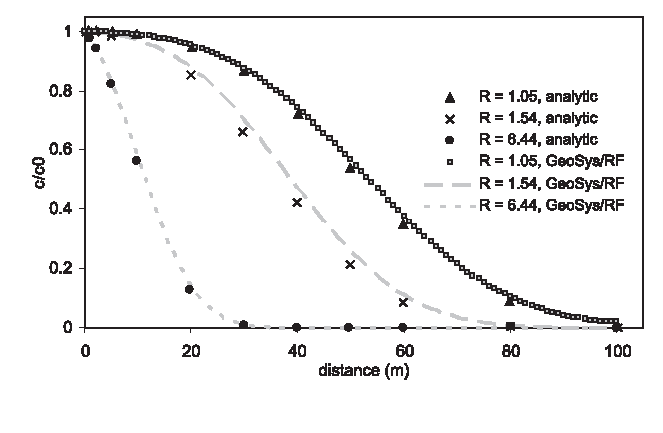
\includegraphics[width=0.8\textwidth]{PART_II/C/fig53.eps}
\caption{Concentration distribution after 100~d (Henry sorption)}
\label{fig53}
\end{figure}

%----------
\subsection{Non-linear sorption (Freundlich isotherm)}

\subsubsection{Definition}

The non-linear Freundlich isotherm is often used to describe real sorption processes. Therefore, in this example, the transport process by including the Freundlich isotherm is calculated in the same way as in the precedent example (same model and boundary conditions). As there exists no opportunity to calculate analytically the solute transport with non-linear sorption, the results of the simulation have to be compared with solutions of the transport equation with linear sorption in order to evaluate the simulation results.

The following simplifications are assumed: (1) non-linear sorption (Freundlich isotherm), no decay of components (2) homogeneous aquifer, saturated, stationary flow (Fig. \ref{fig51}).
%
The soil parameters are the same as listed in Table \ref{tab51}(except decay). For the different simulation runs the Freundlich-sorption coefficients (K$_1$) are varied in the same way as the K$_D$-values that are listed in Table \ref{tab53}. The exponent K$_2$ was constant with a value of 1.

The dependence of sorbed molecules on the amount of molecules in dilution is given by equation (\ref{eq59}). The concentration distribution at a special point in time and over a given distance cannot be calculated analytically by equation (\ref{eq53}) when a non-linear sorption process is assumed. A possibility to test the correctness of the simulation results for transport with Freundlich sorption is to choose values of distribution coefficients in order to create a concentration distribution which is approximately linear and must therefore almost be equal to the results of transport by use of the Henry isotherm.

\subsubsection{Results}

As the values for the Freundlich coefficients were chosen in that way, that the concentration distribution between sorbed and solute concentrations is almost linear, the results of the simulation runs have to be equal to the results that are obtained by using the linear Henry isotherm. In Figure \ref{fig54} the concentration distribution of the solute over the model length of 100~m is shown. As the concentrations of the transport simulation by using the Freundlich isotherm match those of the simulation runs with linear sorption, these results for non-linear sorption are reasonable. Additionally to this test, the values for the constant K$_2$ were changed to 0.8 in order to prove a difference between linear and non-linear sorption. The results of the comparison are shown in Figure \ref{fig55}. These numerical results show the effect of the application of a non-linear sorption isotherm: the higher the influence of sorption (large value of sorption coefficient K$_D$ resp. K$_1$) the higher the difference of solute concentration values between non-linear and linear sorption. However, the results for both isotherms were not evaluated quantitatively.

\begin{figure}[htbp]
\centering
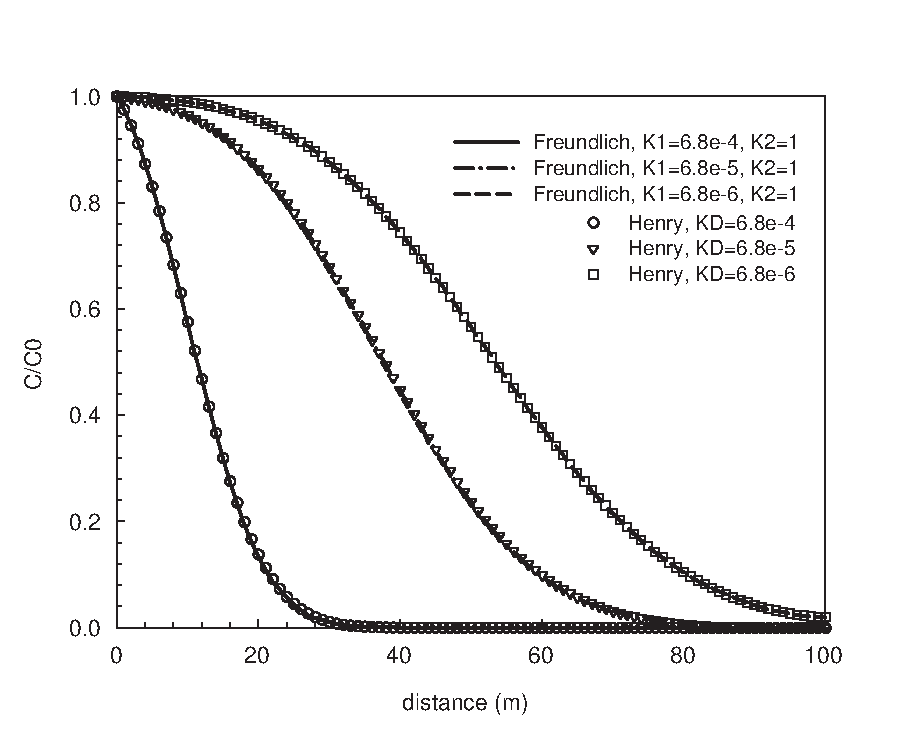
\includegraphics[width=0.8\textwidth]{PART_II/C/fig54.EPS}
\caption{Concentration distribution after 100~d (Freundlich compared to Henry sorption)}
\label{fig54}
\end{figure}

\begin{figure}[htbp]
\centering
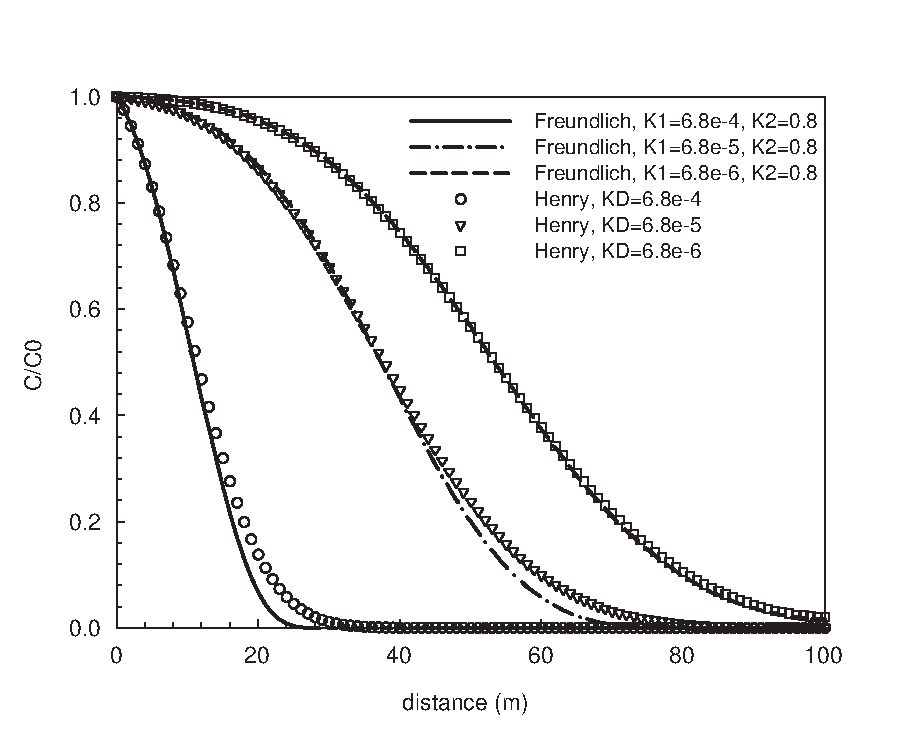
\includegraphics[width=0.8\textwidth]{PART_II/C/fig55.EPS}
\caption{Different concentration distributions after 100~d (Freundlich compared to Henry sorption)}
\label{fig55}
\end{figure}


%----------
\subsection{Non-linear sorption (Langmuir isotherm)}

\subsubsection{Problem definition}

The non-linear Langmuir isotherm is used to describe sorption processes that are restricted by a maximum concentration of sorbed molecules. In this example, the transport process by including the Langmuir isotherm is calculated in the same way as in the precedent examples for mass transport. As there exists no opportunity to calculate analytically the solute transport with non-linear sorption, the results of the simulation have to be compared with solutions of the transport equation with linear sorption in order to evaluate the simulation results.

The following simplifications are assumed: (1) non-linear sorption (Langmuir isotherm), no decay of components (2) homogeneous aquifer, saturated, stationary flow (Fig. \ref{fig51}).
%
The soil parameters are the same as listed in Table \ref{tab51}(except decay). In order to create a Langmuir equation which has almost the same linear characteristic as the Henry equation, the Langmuir sorption coefficients, K$_1$, were varied in the same way as the Henry coefficients (K$_D$ values in Table \ref{tab52}) for the different simulation runs. The K$_2$ coefficients stand for the affinity between solid and sorbed solute. Thus, the K$_2$ value can not be set equal to 0, because this would cause a transport without any sorption. When K$_2$ equals 1, there is no effect on the binding affinity. Therefore, the coefficient K$_2$ was set constant with a value of 1 in order to approximate the linear characteristic of the Henry equation (\ref{eq58}).

The dependence of sorbed molecules on the amount of molecules in dilution is given by equation (\ref{eq510}). The concentration distribution at a special point in time and over a given distance cannot be calculated analytically by equation (\ref{eq53}) when a non-linear sorption process is assumed. Therefore, the simulation results are compared with the results for the mass transport by using the linear Henry isotherm. The non-linear Langmuir isotherm was forced to be almost linear in the way as described above. Now the results of the transport by using the Langmuir isotherm can be compared with the results that were obtained by the transport simulation with the linear Henry isotherm.

\subsubsection{Results}

In Figure \ref{fig56} the concentration distributions over the whole model length by using the linear Henry isotherm and the non-linear Langmuir isotherm are depicted. Obviously, the results for each specified distribution constant are almost equal. This result is correct, because it was provoked by the choice of the sorption coefficients.

\begin{figure}[htbp]
\centering
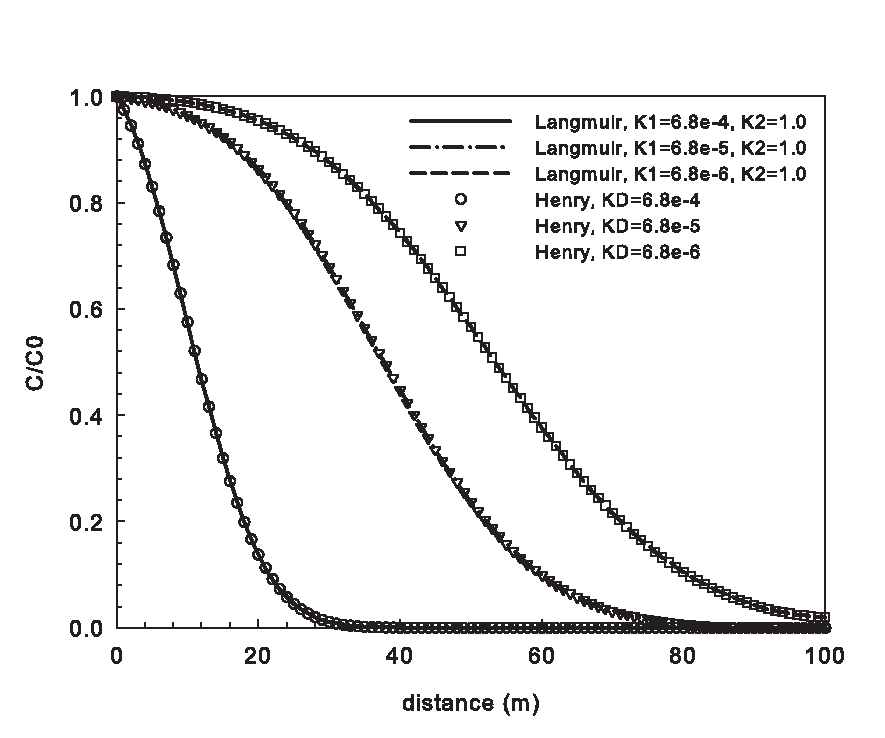
\includegraphics[width=0.8\textwidth]{PART_II/C/fig56.EPS}
\caption{Concentration distribution after 100~d (Langmuir compared to Henry sorption)}
\label{fig56}
\end{figure}

In order to show that the results by the use of the Langmuir isotherm are actually different to those by using the Henry isotherm, the K$_2$ values were changed to a value of 0.8, so that the Langmuir isotherm got a real non-linear gradient. As the results show (Fig. \ref{fig57}), the differences between the concentration distributions are evident.

\begin{figure}[htbp]
\centering
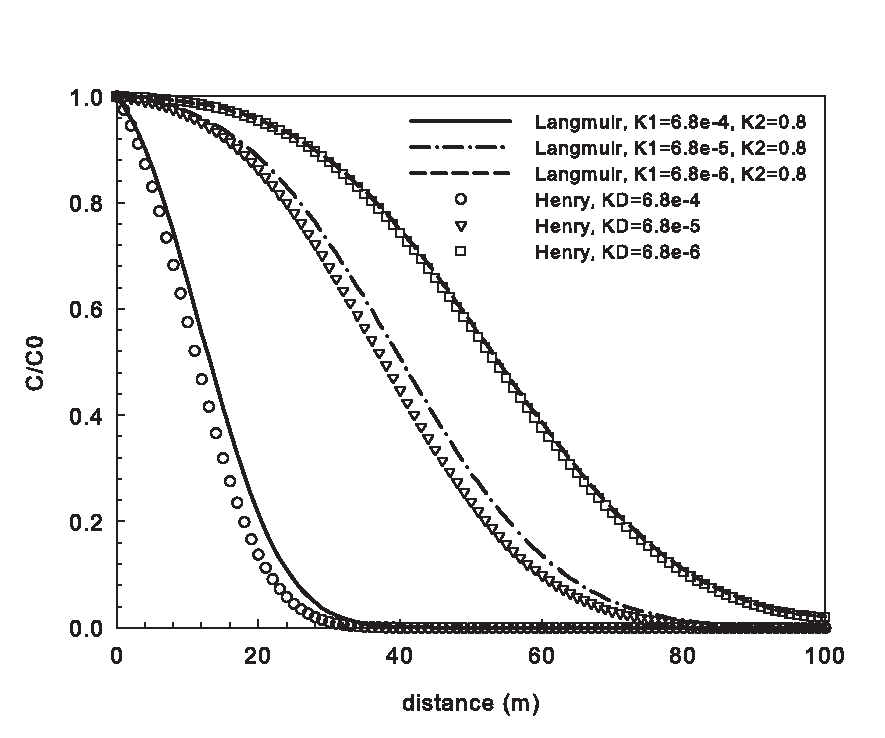
\includegraphics[width=0.8\textwidth]{PART_II/C/fig57.EPS}
\caption{Different concentration distributions after 100~d (Langmuir compared to Henry sorption)}
\label{fig57}
\end{figure}
